\documentclass[11pt, a4paper]{article}
\usepackage[utf8]{inputenc}
\usepackage{graphicx}
\usepackage{float}
\usepackage{pdfpages}
\usepackage{hyperref}
\usepackage{listings}
\usepackage{color}
\usepackage{courier}
\usepackage{multicol}
\usepackage{array}
\usepackage{amsmath}
\usepackage{caption}
\graphicspath{ {./images/} }
\usepackage[margin=2cm]{geometry}
\usepackage{minted}
\usemintedstyle{xcode}
\setminted{breaklines, python3, autogobble, linenos, frame=lines, framesep=2mm}
\hypersetup{
  colorlinks   = true, %Colours links instead of ugly boxes
  urlcolor     = red, %Colour for external hyperlinks
  linkcolor    = black, %Colour of internal links
  citecolor   = blue %Colour of citations
}

\newcommand\MyBox[2]{
  \fbox{\lower0.75cm
    \vbox to 1.7cm{\vfil
      \hbox to 1.7cm{\hfil\parbox{1.4cm}{#1\\#2}\hfil}
      \vfil}%
  }%
}

\begin{document}
    \section{Setup}
        This assignment was written using pipenv for dependency management. Pipenv uses a Pipfile to store dependency information, however a requirements.txt file was also included for convenience.
        \subsection{Requirements}
        The setup assumes you have the following installed:
        \begin{itemize}
            \item python 3.6;
            \item Pipenv or venv.
        \end{itemize}
        The project also depends on the following libraries to run:
        \begin{itemize}
            \item numpy version 1.15;
            \item pandas version 0.23;
            \item matplotlib version 3.0.1.
        \end{itemize}
        \subsection{Installing dependencies Using Pipenv}
            \begin{minted}{bash}
                $ pipenv install # Install dependencies
                $ pipenv shell # Activate Environment
            \end{minted}
        \subsection{Installing Dependencies Using Virtual Environment}
            \begin{minted}{bash}
                $ python3 -m venv venv/ # create virtual Environment
                $ source venv/bin/activate # Activate Environment
                $ pip install -r # Install dependencies
            \end{minted}
    \section{Data Sets}
        \subsection{Types of Test Data}
        \paragraph{} The neural net was challenged with three different datasets:
        \begin{itemize}
            \item A simple problem where the output is (x[0], x[1], x[4])
            \item A normal complexity problem where the output is (x[0] \( \vert \) x[4], x[1] \& x[2], x[4])
            \item A hard problem where the output is (x[0] \( \vert \) x[4], x[1] XOR x[2], x[3] \& x[4])
        \end{itemize}
        \subsection{Running the Data Generation Script}
            For convenience a script was included to automate the generation of test data called generate\_test\_data.py. Data generated will be located in the resources directory. Invoke the following command to generate the test data.
            \begin{listing}[H]
                \begin{minted}{bash}
                    $ chmod +x generate_test_data.py
                    $ ./generate_test_data.py
                \end{minted}
                \caption{Generating the test data}
            \end{listing}
    \section{Neural Net}
        The python script neural\_net contains a class that creates a neural network and implements the error back propagation algorithm.
        \subsubsection{Running the Neural Network}
        Listing~\ref{listing:running_the_nn} demonstrates how to run the neural network.
        \begin{listing}[H]
            \begin{minted}{bash}
                $ chmod +x neural_net.py # change permission to allow execution
                $ ./neural_net.py -h # shows all available arguments.
                $ ./neural_net.py --dataset simple_problem # trains the network for the simple_problem dataset for 1000 epochs
                $ ./neural_net.py --dataset hard_problem --epochs 4000 # trains the  network on the hard_problem dataset for 4000 epochs
            \end{minted}
            \caption{Running the Neural Network}
            \label{listing:running_the_nn}
        \end{listing}
        \subsection{Results}
            For convenience the script outputs a confusion matrix with the associated statistics to measure the neural net's performance. The matrix is represented as follows: 
            \[
                \begin{bmatrix}
                    TP & FN \\
                    FP & TN
                \end{bmatrix}
            \]
            \subsubsection{Simple Problem}
            \paragraph{}Figure~\ref{fig:simple_problem_perf} shows the performance of the neural net on the simple problem dataset.
            \begin{figure}[H]
                \centering
                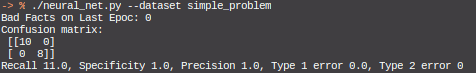
\includegraphics[width=0.9\textwidth, keepaspectratio]{simple_problem_stats.png}
                \caption{Simple problem performance.}
                \label{fig:simple_problem_perf}
            \end{figure}
            \paragraph{}Figure~\ref{fig:simple_problem_bad_epoch} shows  a graph of the bad facts against epochs on the simple problem dataset.
            \begin{figure}[H]
                \centering
                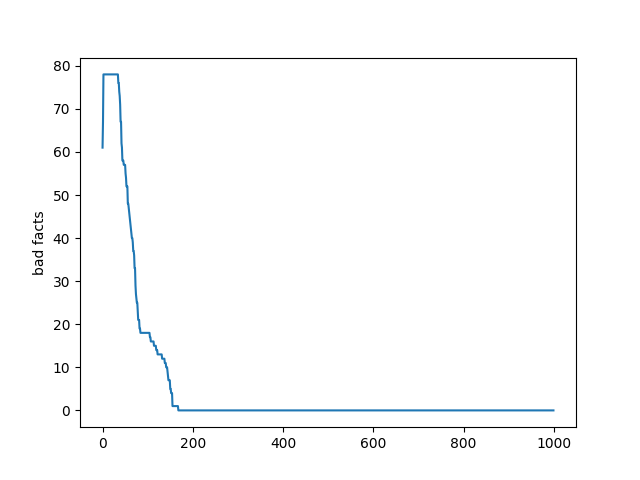
\includegraphics[width=0.9\textwidth, keepaspectratio]{simple_problem.png}
                \caption{Graph of Bad facts vs Epoch.}
                \label{fig:simple_problem_bad_epoch}
            \end{figure}

            \subsubsection{Normal Problem}
            \paragraph{}Figure~\ref{fig:normal_problem_perf} shows the performance of the neural net on the normal problem dataset.
            \begin{figure}[H]
                \centering
                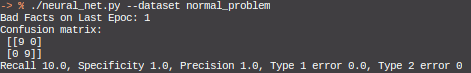
\includegraphics[width=0.9\textwidth, keepaspectratio]{normal_problem_stats.png}
                \caption{Normal problem performance.}
                \label{fig:normal_problem_perf}
            \end{figure}
            \paragraph{}Figure~\ref{fig:normal_problem_bad_epoch} shows  a graph of the bad facts against epochs on the normal problem dataset.
            \begin{figure}[H]
                \centering
                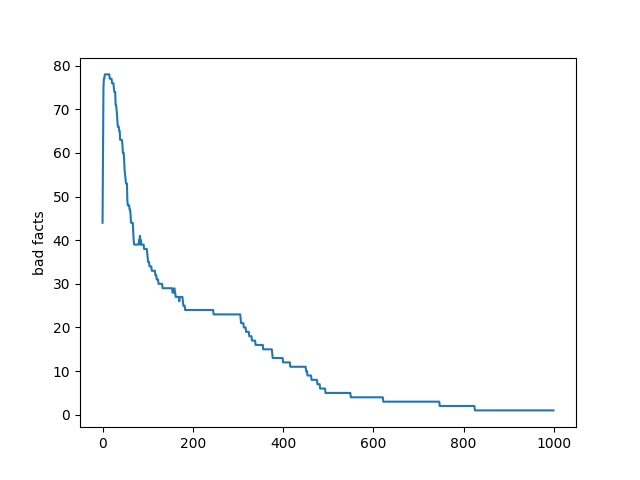
\includegraphics[width=0.9\textwidth, keepaspectratio]{normal_problem.png}
                \caption{Graph of Bad facts vs Epoch for the normal dataset.}
                \label{fig:normal_problem_bad_epoch}
            \end{figure}

            \subsubsection{Hard Problem}
            \paragraph{}Figure~\ref{fig:hard_problem_perf} shows the performance of the neural net on the hard problem dataset.
            \begin{figure}[H]
                \centering
                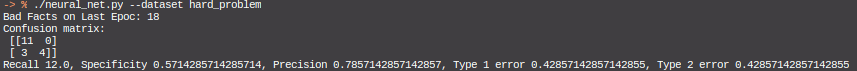
\includegraphics[width=0.9\textwidth, keepaspectratio]{hard_problem_stats.png}
                \caption{Hard problem performance.}
                \label{fig:hard_problem_perf}
            \end{figure}
            \paragraph{}Figure~\ref{fig:hard_problem_bad_epoch} shows  a graph of the bad facts against epochs on the hard problem dataset.
            \begin{figure}[H]
                \centering
                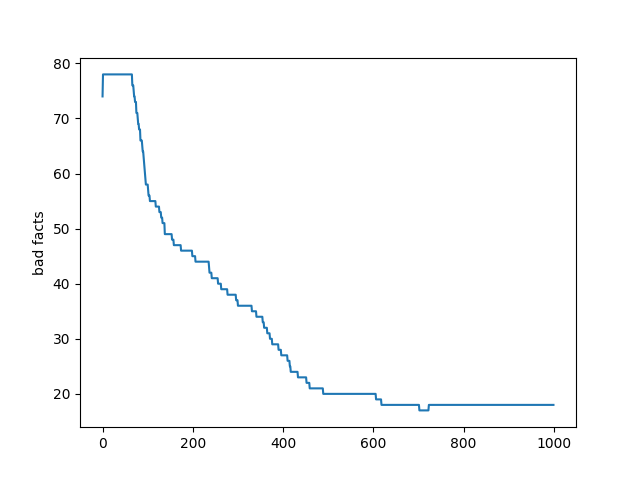
\includegraphics[width=0.9\textwidth, keepaspectratio]{hard_problem.png}
                \caption{Graph of Bad facts vs Epoch for the hard dataset.}
                \label{fig:hard_problem_bad_epoch}
            \end{figure}
    \section{Code}
    \subsection{Csv Utils Script}
    \paragraph{} A class dedicated to manipulate CSV files was created called csv\_utils.
    \inputminted{python}{../utils/csv_utils.py}
    \subsection{Generate Data Script}
    \paragraph{} An executable script to generate test data.
    \inputminted{python}{../generate_test_data.py}
    \captionof{listing}{Generate test Data}
    \subsection{Neural Network Script}
    \paragraph{} An executable script that implements the error back propagation algorithm.
    \inputminted{python}{../neural_net.py}
    \captionof{listing}{Neural Network}
\end{document}